\documentclass{article}
\usepackage[margin=0.8in]{geometry} % change this parameter to enlarge/restrict the margins
\usepackage{amsmath,amsthm,amssymb,amsfonts, fancyhdr, color, comment, graphicx, environ}
\usepackage{xcolor}
\usepackage{mdframed}
\usepackage[shortlabels]{enumitem}
\usepackage{hyperref}
\usepackage{calrsfs}
\DeclareMathAlphabet{\pazocal}{OMS}{zplm}{m}{n}
\usepackage{graphicx}
\usepackage{makecell} %table cells
\usepackage{booktabs} %table appearance
\usepackage{caption} %table caption

\renewcommand{\footrulewidth}{0.8pt}
\hypersetup{
	colorlinks=true,
	linkcolor=blue,
	filecolor=magenta,      
	urlcolor=blue,
}

%/ Margin
%/ ##########################
%/\addtolength{\oddsidemargin}{-.7in}
%/\addtolength{\evensidemargin}{-.7in}
%/\addtolength{\textwidth}{1.4in} %/Double of the 2 above
% ###########################

% fancy style 
\pagestyle{fancy}
% remove fancy style from bottom 
\renewcommand{\footrulewidth}{0pt}

\lhead{Group 20}
\rhead{Algorithmic Machine Learning} 

\newcommand{\loss}{L(\theta, a)}
\newcommand{\lossRule}{L(\theta, \delta(x))}
\newcommand{\risk}{R(\theta, \delta)}

%------------------------------------------------
% Bibliography
\usepackage[sorting=none, backend=bibtex]{biblatex}
\addbibresource{ref.bib}
%------------------------------------------------


\begin{document}
	\title{\Large Algorithmic Machine Learning  \\[0.5cm]
	\bf\Large Challenge 1 - Report \\[0.5cm]
	
	\bf\Large Group 20}

\author{\large 
	\begin{tabular}{rl}
		\textbf{Professor:} & Pietro Michiardi \\
		\textbf{Authors:} & Daniele Falcetta \\ & Simone Papicchio \\ & Massimiliano Pronesti \\ & Federico Tiblias
	\end{tabular}
	}
\date{\large \today}

\makeatletter
\begin{titlepage}
	\begin{center}
		{ 
\includegraphics[width=10cm]{assets/eurecom.png}}
		{\ \\ \ \\}
		\vbox{}\vspace{5cm}
		{\@title }\\[3cm]
		{\@author}\\[3cm]
		{\@date\\}
		
	\end{center}
\end{titlepage}
\makeatother
	
\section{Introduction}
Sentiment analysis is a rapidly growing field, as large databases become increasingly available, and companies have an interest in automatically extracting sentiment from internet users.

With the increasing amount of content and debate on social media platforms such as Twitter, there is an interest in automatically extracting meaning and sentiment from users' posts, to be able to evaluate the aggregate opinion of a large number of users. Capturing sentiment in language is important in these times where decisions and reactions are created and updated in seconds.

The dataset used for this challenge consist of tweets from Figure Eight's Data for Everyone platform. The main task is to classify tweets with positive, neutral, or negative labels, reflecting the sentiment of the user writing the tweet.

Our approaches ...............

In this challenge we also address a further bonus task which consists of detecting the relevant words inside the tweet which are most responsible for the attributed sentiment.

Our approach for the bonus .........................

\section{Data Analysis \& Pre-processing}
    \subsection{Data exploration}

    \subsection{Transformations}
	\begin{itemize}
		\item \textbf{Stopword removal:}
		\item \textbf{...}
		\item \textbf{Word2Vec:}
		\item \textbf{Data Augmentation:} In order to give more variety to the model, we build new tweets by concatenating existing ones. Couples are formed randomly and kept only if A) the tweets have the same label and B) the resulting tweet is $< 140$ characters long. This procedure can be repeated producing datasets of increasing size.
	\end{itemize}


\section{Models}
    Transformers are undoubtedly the gold standard for many NLP tasks including sentiment analysis. Nevertheless, we also try different approaches to see how they compare  with the state of the art.
    
    Performances are computed by first splitting the labelled data in development and validation datasets (80/20 random split), then training on the development part, and finally assessing performances on the unseen validation subset. If the model reaches satisfying performances is then applied on the unlabelled test dataset and predictions are uploaded on Kaggle.

	\begin{itemize}
		\item \textbf{Word2Vec + CatBoost:}
		\item \textbf{LSTM:}
		\item \textbf{...}
	\end{itemize}

  \begin{figure}
    \centering
    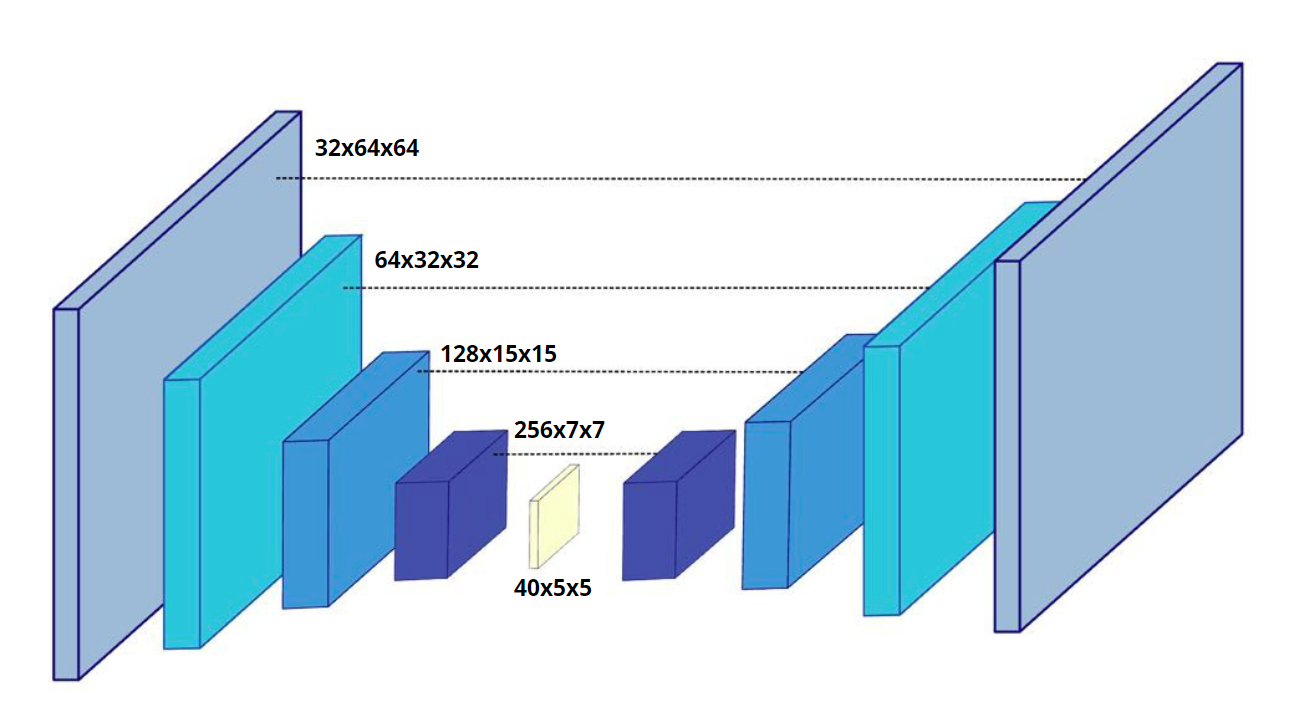
\includegraphics[width=.7\linewidth]{assets/cnnAE.png}
    \caption{ aaa }
    \label{fig:cnnAE}
\end{figure}


\section{Results}

\section{Conclusions}

%% display bibliography at the end
\printbibliography
\end{document}